% !Mode:: "TeX:UTF-8"
% 请注意,此文件的编码方式一定要设置为UTF-8 无DOM模式
% 否则中文显示乱码!
% 可以用notepad++ 或ultraedit查看/更改文件编码方式

\documentclass[a4paper,12pt]{article}

%插入超链接,并且去除超链接的颜色下划线等特性
\usepackage[hidelinks]{hyperref}

%该宏包可以添加伪代码CLRS《算法导论》**第三版**模式
%clrscode3e.sty放在项目根目录下即可
\usepackage{clrscode3e}

%插入数学公式
\usepackage{amsmath}

%https://www.sharelatex.com/learn/Theorems_and_proofs
\newtheorem{theorem}{Theorem}[section]
\newtheorem{corollary}{Corollary}[theorem]
\newtheorem{lemma}[theorem]{Lemma}

%中文包
\usepackage{xeCJK}
\setCJKmainfont{SimSun}

%设置页边距
\usepackage[top=1in,bottom=0.8in,left=1.1in,right=1in]{geometry}

\usepackage{xcolor}

%为了插入代码
\usepackage{listings}

\definecolor{codegreen}{rgb}{0,0.6,0}
\definecolor{codegray}{rgb}{0.5,0.5,0.5}
\definecolor{codepurple}{rgb}{0.58,0,0.82}
\definecolor{backcolour}{rgb}{0.95,0.95,0.92}

\lstdefinestyle{mystyle}{
    backgroundcolor=\color{backcolour},
    commentstyle=\itshape\color{codegreen},
    keywordstyle=\color{magenta},
    numberstyle=\tiny\color{codegray},
    stringstyle=\color{codepurple},
    basicstyle=\footnotesize,
    breakatwhitespace=false,
    breaklines=true,
    captionpos=b,
    keepspaces=true,
    numbers=left,
    numbersep=5pt,
    showspaces=false,
    showstringspaces=false,
    showtabs=false,
    tabsize=4
}

\lstdefinestyle{default}{
    commentstyle=\itshape,
    numberstyle=\tiny,
    basicstyle=\footnotesize,
    breakatwhitespace=false,
    breaklines=true,
    captionpos=b,
    keepspaces=true,
    numbers=left,
    numbersep=5pt,
    showspaces=false,
    showstringspaces=false,
    showtabs=false,
    tabsize=4
}

\lstset{style=mystyle}

%为了插入图片
%\usepackage{graphicx}

%为了画图
\usepackage{tikz}
\usetikzlibrary{positioning}

%首段缩进
\usepackage{indentfirst}

\title{Assignment 3 Supplement\\Algorithm Design and Analysis}

\author{\href{http://bitjoy.net}{bitjoy.net}}
\date{January 13, 2016}

\begin{document}

\maketitle

\section*{1\quad Greedy Algorithm}
给定一系列自然数$d_1\geq d_2\geq ...\geq d_n\geq 0$,如果存在一个图,其每个顶点的度数分别是$d_1,d_2,...,d_n$,当且仅当存在另一个图,其每个顶点的度数分别为$d_2-1,d_3-1,...,d_{d_1+1}-1,d_{d_1+2},...,d_n$。

下面我们来证明这个定理。

$\Leftarrow$ 如果存在一个图,其每个顶点的度数分别为$d_2-1,d_3-1,...,d_{d_1+1}-1,d_{d_1+2},...,d_n$,则我们添加一个顶点$v_1$,将$v_1$和后面$d_1$个点都连一条边,则新的图中,顶点$v_1,v_2,...,v_n$的度数分别为$d_1,d_2,...,d_n$。


$\Rightarrow$ 如果存在一个图,其每个顶点的度数分别为$d_1,d_2,...,d_n$,且满足$d_1\geq d_2\geq ...\geq d_n\geq 0$,则$v_1$恰和后面$d_1$个顶点都有一条边。如果把$v_1$及其$d_1$条边删掉,则形成了一个顶点度数分别为$d_2-1,d_3-1,...,d_{d_1+1}-1,d_{d_1+2},...,d_n$的图。

假设存在某个点$i\in[2,d_1+1]$和$v_1$没有边,则$v_1$为了凑够$d_1$条边,必须和某个点$j\in[d_1+2,n]$有一条边。同时因为$d_i\geq d_j$,必存在一个点$k$,$v_i$连了但$v_j$没连。所以我们删除边$(v_i,v_k)$和$(v_1,v_j)$,添加上边$(v_1,v_i)$和$(v_j,v_k)$,则每个顶点的度数都没有改变,但$v_1$和其后$d_1$个顶点都有了连边。所以上面证明的第二步成立。

%http://tex.stackexchange.com/questions/8652/what-does-t-and-ht-mean
\begin{figure}[!ht]
\centering
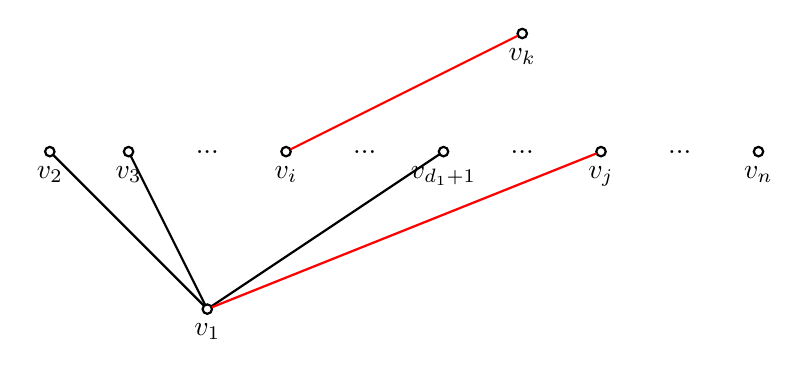
\begin{tikzpicture}
    [empty/.style={circle, draw=black,thick,inner sep=0pt,minimum size=6mm,scale=0.2}]
    \node[empty,label=below:{$v_1$}] (v1) at (2,-2) {};
    \node[empty,label=below:{$v_k$}] (vk) at (6,1.5) {};
    \node[empty,label=below:{$v_2$}] (v2) at (0,0) {};
    \node[empty,label=below:{$v_3$}] (v3) at (1,0) {};
    \node[] (none1) at (2,0) {...};
    \node[empty,label=below:{$v_i$}] (vi) at (3,0) {};
    \node[] (none2) at (4,0) {...};
    \node[empty,label=below:{$v_{d_1+1}$}] (vd1p1) at (5,0) {};
    \node[] (none3) at (6,0) {...};
    \node[empty,label=below:{$v_j$}] (vj) at (7,0) {};
    \node[] (none4) at (8,0) {...};
    \node[empty,label=below:{$v_n$}] (vn) at (9,0) {};

    \draw [black,thick] (v1) -- (v2);
    \draw [black,thick] (v1) -- (v3);
    \draw [black,thick] (v1) -- (vd1p1);
    \draw [red,thick] (v1) -- (vj);
    \draw [red,thick] (vi) -- (vk);
\end{tikzpicture}
\caption{原图$G$,$v_1$并没有和其后$d_1$个点都有边。}
\end{figure}

%http://tex.stackexchange.com/questions/8652/what-does-t-and-ht-mean
\begin{figure}[!ht]
\centering
\begin{tikzpicture}
    [empty/.style={circle, draw=black,thick,inner sep=0pt,minimum size=6mm,scale=0.2}]
    \node[empty,label=below:{$v_1$}] (v1) at (2,-2) {};
    \node[empty,label=below:{$v_k$}] (vk) at (6,1.5) {};
    \node[empty,label=below:{$v_2$}] (v2) at (0,0) {};
    \node[empty,label=below:{$v_3$}] (v3) at (1,0) {};
    \node[] (none1) at (2,0) {...};
    \node[empty,label=below:{$v_i$}] (vi) at (3,0) {};
    \node[] (none2) at (4,0) {...};
    \node[empty,label=below:{$v_{d_1+1}$}] (vd1p1) at (5,0) {};
    \node[] (none3) at (6,0) {...};
    \node[empty,label=below:{$v_j$}] (vj) at (7,0) {};
    \node[] (none4) at (8,0) {...};
    \node[empty,label=below:{$v_n$}] (vn) at (9,0) {};

    \draw [black,thick] (v1) -- (v2);
    \draw [black,thick] (v1) -- (v3);
    \draw [black,thick] (v1) -- (vd1p1);
    \draw [blue,thick] (v1) -- (vi);
    \draw [blue,thick] (vj) -- (vk);
\end{tikzpicture}
\caption{转换后的图$G'$,$v_1$和其后$d_1$个点都有边,$G'$和$G$等价。}
\end{figure}

\begin{codebox}
\Procname{$\proc{GRAPH-EXISTING}(D)$}
\li \If $D=NULL$
    \Then
\li \Return true
    \End
\li sort $D$ in descending order
\li remove $d_1$ from $D$
\li \For $i$ = 2 \To $d_1+1$
    \Do
\li $d_i=d_i-1$
\li \If $d_i<0$
    \Then
\li \Return false
\li \ElseIf $d_i==0$
    \Then
\li remove $d_i$ from $D$
    \End
    \End
\li \Return GRAPH-EXISTING(D)
\end{codebox}

时间复杂度为$O(n^2logn)$。

\section*{4\quad Greedy Algorithm}
和第3题类似,分别把A和B从大到小排序,然后把$a_i$和$b_i$配对,得到的$\prod\limits_{i=1}^{n}a_i^{b_i}$最大。

使用\emph{exchange argument}证明如下:

假设用该算法得到的解为$S$,对于另一个解$S'\neq S$,必存在某两对$(a_i,b_i)$和$(a_j,b_j)$,他们是逆序对,即$a_i\geq a_j$且$b_i\leq b_j$,乘积为$T'=a_i^{b_i}a_j^{b_j}$。如果交换这两对,使得$(a_i,b_j)$和$(a_j,b_i)$,消除了逆序对,新的乘积为$T=a_i^{b_j}a_j^{b_i}$,我们要证明$T\geq T'$。

\[
\frac{T}{T'}=\frac{a_i^{b_j}a_j^{b_i}}{a_i^{b_i}a_j^{b_j}}=a_i^{b_j-b_i}a_j^{b_i-b_j}=(\frac{a_i}{a_j})^{b_j-b_i}\geq 1
\]
所以$T\geq T'$。也就是说,由$S'$转换到$S$的过程中,并没有减小乘积,所以$S$是最优解。
\end{document}
